\documentclass[xcolor=dvipsnames]{beamer}
\usetheme{Madrid}
\usecolortheme[named=NavyBlue]{structure}
% \colorlet{beamer@blendedblue}{green!40!black}
\usepackage{graphicx}
\usepackage{caption}
\usepackage{siunitx}
\usepackage{circuitikz}

\newcommand{\important}[1]{\textcolor{structure.fg}{\textit{#1}}}

\title{Thevenin's Theorem}
\author{Paul John Placer}
\date{June 10, 2026}


\begin{document}
    \frame{\titlepage}

    \begin{frame}{Introduction}
        \begin{block}{Thevenin's Theorem}
            Any \important{linear circuit} can be simplified into an \important{equivalent circuit} consisting of a single voltage source and series resistance connected to a load. \medbreak

            This simplification allows for easily analyzing the effect of the circuit on different loads without having to recalculate with the whole circuit for each load.
        \end{block} \vspace{1.25em}

        \footnotesize A \textit{linear circuit} is a circuit consisting of only linear components: resistors, capacitors, and inductors; their voltage-current relationship is linear.
    \end{frame}

    \begin{frame}{Introduction}
        \begin{figure}[h]
            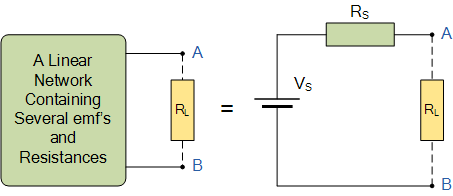
\includegraphics[scale=0.5]{images/thevenin_equivalent.png}
            \centering
            \caption*{\footnotesize{Source: \href{https://www.ilearnengineering.com/electronical-and-electronic/how-do-we-apply-thevenins-theorem}{ilearnengineering.com}}}
        \end{figure}
    \end{frame}

    \begin{frame}{Introduction}
        \begin{block}{Thevenin Equivalent}
            The Thevenin equivalent circuit of any given circuit consists of the \important{Thevenin voltage $V_{Th}$} and the \important{Thevenin resistance $R_{Th}$}, all in series with the load component (usually modeled as a load resistor $R_L$). \medbreak

            To solve for $V_{Th}$ and $R_{Th}$, first \important{disconnect the load}. These values can then be solved for by viewing the circuit through the resulting \important{open terminals} from the disconnected load.
        \end{block}
    \end{frame}

    \begin{frame}{Thevenin Equivalent}
        \begin{block}{Thevenin Voltage}
            The Thevenin voltage $V_{Th}$ is obtained by calculating the voltage between open terminals \important{A} and \important{B}.
        \end{block}

        \begin{block}{Thevenin Resistance}
            The Thevenin resistance $R_{Th}$ is obtained by zeroing all independent sources and then calculating the equivalent resistance of the resulting circuit as seen from open terminals \important{A} and \important{B}.
        \end{block}
    \end{frame}

    \begin{frame}{Example}
        Using Thevenin's Theorem, determine the voltage across $R_L$: \bigbreak

        \begin{figure}[h]
            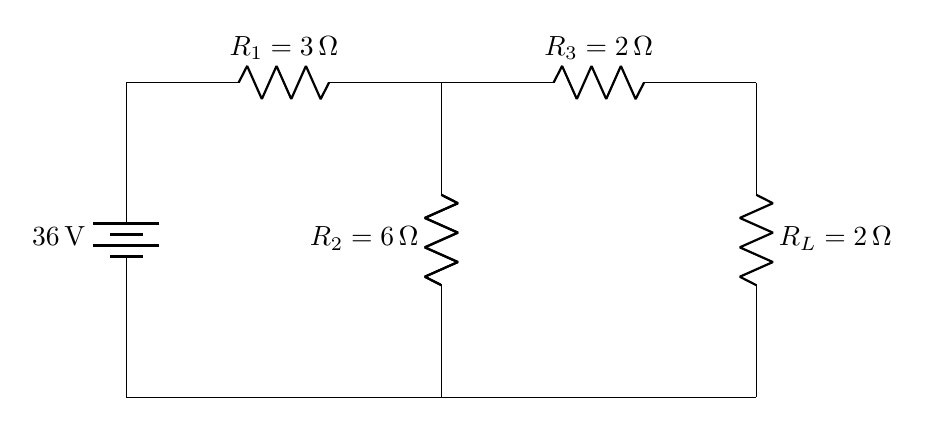
\begin{tikzpicture}[transform shape]
                % Paths, nodes and wires:
                \draw (-4, 2) to[battery, l_={$\qty{36}{\volt}$}] (-4, -2);
                \draw (-4, 2) to[american resistor, l={$R_1 = \qty{3}{\ohm}$}] (0, 2);
                \draw (0, 2) to[american resistor] (0, -2);
                \draw (-4, -2) to[short] (0, -2);
                \draw (0, 2) to[american resistor, l={$R_3 = \qty{2}{\ohm}$}] (4, 2);
                \draw (0, 2) to[american resistor, l_={$R_2 = \qty{6}{\ohm}$}] (0, -2);
                \draw (4, 2) to[american resistor, l={$R_L = \qty{2}{\ohm}$}] (4, -2);
                \draw (0, -2) to[short] (4, -2);
            \end{tikzpicture}
        \end{figure}
    \end{frame}

    \begin{frame}{Example}
        Solving for $V_{Th}$: \bigbreak

        \begin{figure}[h]
            \hspace{-0.75cm}
            \scalebox{0.75}{\begin{tikzpicture}[transform shape]
                % Paths, nodes and wires:
                \draw (-4, 2) to[battery, l_={$\qty{36}{\volt}$}] (-4, -2);
                \draw (-4, 2) to[american resistor, l={$R_1 = \qty{3}{\ohm}$}] (0, 2);
                \draw (0, 2) to[american resistor] (0, -2);
                \draw (-4, -2) to[short] (0, -2);
                \draw (0, 2) to[american resistor, l={$R_3 = \qty{2}{\ohm}$}] (4, 2);
                \draw (0, 2) to[american resistor, l_={$R_2 = \qty{6}{\ohm}$}] (0, -2);
                \draw (-0, -2) to[short] (4, -2);
                \node[ocirc](N1) at (4, 2){} node[anchor=west] at (N1.east){$A$};
                \node[ocirc](N2) at (4, -2){} node[anchor=west] at (N2.east){$B$};
            \end{tikzpicture}}
        \end{figure}
        % \[V_{Th} = V_{R_2} \quad V_{R_2} = \frac{}{}\]
        \begin{align*}
            \onslide<2->{V_{Th} &= V_{R_2} \\}
            \onslide<3->{       &= \qty{36}{\volt} \frac{\qty{6}{\ohm}}{\qty{3}{\ohm} + \qty{6}{\ohm}} \\}
            \onslide<4->{       &= \qty{24}{\volt}}
        \end{align*}
    \end{frame}

    \begin{frame}{Example}
        Solving for $R_{Th}$:

        \begin{figure}[h]
            \scalebox{0.75}{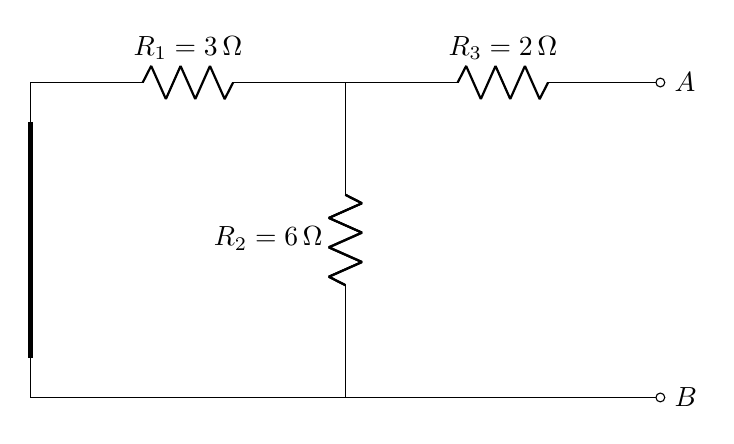
\begin{tikzpicture}[transform shape]
            % Paths, nodes and wires:
                \draw (-4, 2) to[american resistor, l={$R_1 = \qty{3}{\ohm}$}] (0, 2);
                \draw (0, 2) to[american resistor] (0, -2);
                \draw (-4, -2) to[short] (0, -2);
                \draw (0, 2) to[american resistor, l={$R_3 = \qty{2}{\ohm}$}] (4, 2);
                \draw (0, 2) to[american resistor, l_={$R_2 = \qty{6}{\ohm}$}] (0, -2);
                \draw (-0, -2) to[short] (4, -2);
                \node[ocirc](N1) at (4, 2){} node[anchor=west] at (N1.east){$A$};
                \node[ocirc](N2) at (4, -2){} node[anchor=west] at (N2.east){$B$};
                \draw (-4, 2) to[short] (-4, -2);
                \draw[line width=2pt] (-4, 1.5) -- (-4, -1.5);
            \end{tikzpicture}}
        \end{figure}

        \begin{align*}
            \onslide<2->{R_{Th} &= \qty{3}{\ohm}\parallel\qty{6}{\ohm} + \qty{2}{\ohm} \\}
            \onslide<3->{       &= \qty{2}{\ohm} + \qty{2}{\ohm} \\}
            \onslide<4->{       &= \qty{4}{\ohm}}
        \end{align*}
    \end{frame}

    \begin{frame}{Example}
        The resulting Thevenin equivalent circuit:

        \begin{figure}[h]
            \scalebox{0.75}{\begin{tikzpicture}[transform shape]
                % Paths, nodes and wires:
                \draw (-2, 2) to[battery, l_={$V_{Th} = \qty{24}{\volt}$}] (-2, -2);
                \draw (-2, 2) to[american resistor, l={$R_{Th} = \qty{4}{\ohm}$}] (2, 2);
                \draw (-2, -2) -- (2, -2);
                \node[ocirc](N1) at (2, 2){} node[anchor=west] at (N1.east){$A$};
                \node[ocirc](N2) at (2, -2){} node[anchor=west] at (N2.east){$B$};
                \draw (2, 2) to[american resistor, o-o, l={$R_L = \qty{2}{\ohm}$}] (2, -2);
            \end{tikzpicture}}
        \end{figure}

        \onslide<2->{$V_{R_L}$ becomes a simple \important{voltage divider}:}
        \begin{align*}
            \onslide<2->{V_{R_L} &= V_{Th} \frac{R_L}{R_{Th} + R_L} \\}
            \onslide<3->{        &= \qty{24}{\volt} \frac{\qty{2}{\ohm}}{\qty{4}{\ohm} + \qty{2}{\ohm}} \\}
            \onslide<4->{        &= \qty{8}{\volt}}
        \end{align*}
    \end{frame}

    \begin{frame}{Example - Bridge Circuit}
        Find the Thevenin equivalent of the circuit below: \bigbreak

        \begin{figure}[h]
            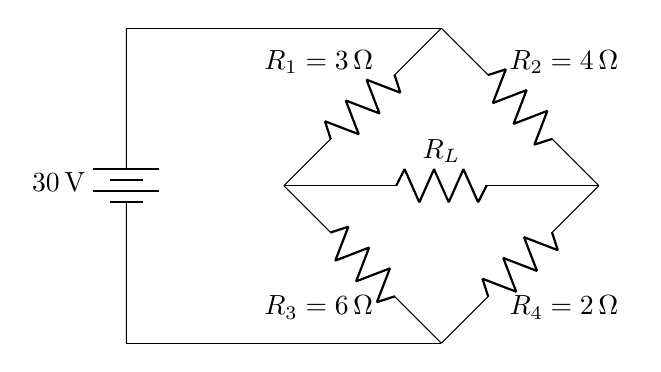
\begin{tikzpicture}[transform shape]
                \ctikzset{label/align=straight}
                % Paths, nodes and wires:
                \draw (-3, 2) to[battery, l_={$\qty{30}{\volt}$}] (-3, -2);
                \draw (1, 2) to[american resistor, l_={$R_1 = \qty{3}{\ohm}$}, label distance=0.25cm] (-1, -0);
                \draw (3, 0) to[american resistor, l_={$R_2 = \qty{4}{\ohm}$}, label distance=0.25cm] (1, 2);
                \draw (3, 0) to[american resistor, l_={$R_L$}] (-1, 0);
                \draw (1, -2) to[american resistor, l={$R_3 = \qty{6}{\ohm}$}, label distance=0.25cm] (-1, 0);
                \draw (3, 0) to[american resistor, l={$R_4 = \qty{2}{\ohm}$}, label distance=0.25cm] (1, -2);
                \draw (-3, 2) -- (1, 2);
                \draw (-3, -2) -- (1, -2);
            \end{tikzpicture}
        \end{figure}
    \end{frame}

    \begin{frame}{Example - Bridge Circuit}
        Solving for $V_{Th}$:

        \begin{figure}[h]
            \scalebox{0.75}{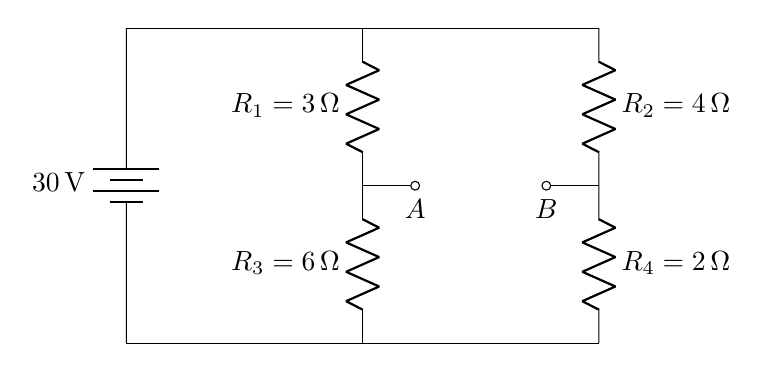
\begin{tikzpicture}[transform shape]
                % Paths, nodes and wires:
                \draw (-3, 2) to[battery, l_={$\qty{30}{\volt}$}] (-3, -2);
                \draw (0, 2) to[american resistor, l_={$R_1 = \qty{3}{\ohm}$}] (0, -0);
                \draw (3, -0) to[american resistor, l_={$R_2 = \qty{4}{\ohm}$}] (3, 2);
                \draw (0, -2) to[american resistor, l={$R_3 = \qty{6}{\ohm}$}] (0, 0);
                \draw (3, -0) to[american resistor, l={$R_4 = \qty{2}{\ohm}$}] (3, -2);
                \draw (-3, 2) -- (3, 2);
                \draw (-3, -2) -- (3, -2);
                \draw (0, -0) -- (0.667, -0);
                \draw (3, -0) -- (2.333, -0);
                \node[ocirc](N1) at (0.667, -0){} node[anchor=north] at (N1.south){$A$};
                \node[ocirc](N2) at (2.333, -0){} node[anchor=north] at (N2.south){$B$};
            \end{tikzpicture}}
        \end{figure}

        \begin{align*}
            \onslide<2->{V_{Th} &= V_A - V_B \\}
            \onslide<3->{       &= \frac{\qty{30}{\volt} \cdot \qty{6}{\ohm}}{\qty{3}{\ohm} + \qty{6}{\ohm}} - \frac{\qty{30}{\volt} \cdot \qty{2}{\ohm}}{\qty{4}{\ohm} + \qty{2}{\ohm}} \\}
            \onslide<4->{       &= \qty{20}{\volt} - \qty{10}{\volt} \\}
            \onslide<5->{       &= \qty{10}{\volt}}
        \end{align*}
    \end{frame}

    \begin{frame}{Example - Bridge Circuit}
        Solving for $R_{Th}$:

        \begin{overlayarea}{\textwidth}{0.375\textheight}
            \only<1>{
                \begin{figure}[h]
                    \hspace{0.75cm}
                    \scalebox{0.75}{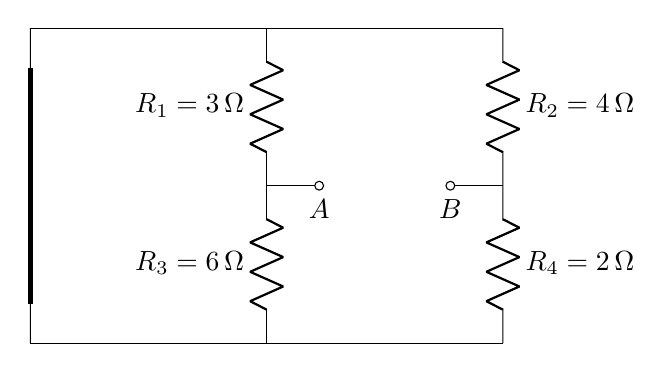
\begin{tikzpicture}[transform shape]
                        % Paths, nodes and wires:
                        \draw (0, 2) to[american resistor, l_={$R_1 = \qty{3}{\ohm}$}] (0, -0);
                        \draw (3, -0) to[american resistor, l_={$R_2 = \qty{4}{\ohm}$}] (3, 2);
                        \draw (0, -2) to[american resistor, l={$R_3 = \qty{6}{\ohm}$}] (0, -0);
                        \draw (3, -0) to[american resistor, l={$R_4 = \qty{2}{\ohm}$}] (3, -2);
                        \draw (-3, 2) -- (3, 2);
                        \draw (-3, -2) -- (3, -2);
                        \draw (0, -0) -- (0.667, -0);
                        \draw (3, -0) -- (2.333, -0);
                        \node[ocirc](N1) at (0.667, -0){} node[anchor=north] at (N1.south){$A$};
                        \node[ocirc](N2) at (2.333, -0){} node[anchor=north] at (N2.south){$B$};
                        \draw (-3, 2) to[short] (-3, -2);
                        \draw[line width=2pt] (-3, 1.5) -- (-3, -1.5);
                    \end{tikzpicture}}
                \end{figure}
            }

            \only<2->{
                \begin{figure}[h]
                    \scalebox{0.75}{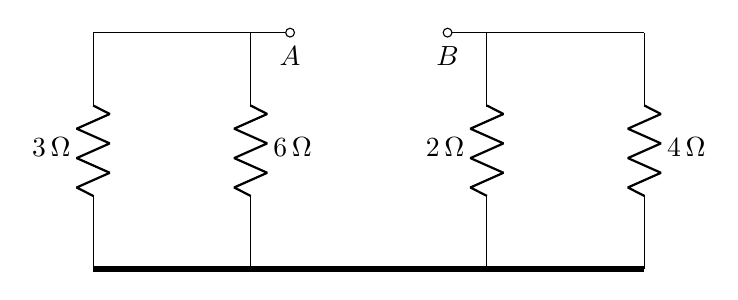
\begin{tikzpicture}[transform shape]
                        % Paths, nodes and wires:
                        \draw (-3.5, 1.5) to[american resistor, l_={$\qty{3}{\ohm}$}] (-3.5, -1.5);
                        \draw (3.5, -1.5) to[american resistor, l_={$\qty{4}{\ohm}$}] (3.5, 1.5);
                        \draw (-1.5, -1.5) to[american resistor, l_={$\qty{6}{\ohm}$}] (-1.5, 1.5);
                        \draw (1.5, 1.5) to[american resistor, l_={$\qty{2}{\ohm}$}] (1.5, -1.5);
                        \draw[line width=2pt] (-3.5, -1.5) -- (3.5, -1.5);
                        \draw (-3.5, 1.5) -- (-1, 1.5);
                        \draw (1, 1.5) -- (3.5, 1.5);
                        \node[ocirc](N1) at (-1, 1.5){} node[anchor=north] at (N1.south){$A$};
                        \node[ocirc](N2) at (1, 1.5){} node[anchor=north] at (N2.south){$B$};
                    \end{tikzpicture}}
                \end{figure}
            }
        \end{overlayarea}

        \begin{align*}
            \onslide<3->{R_{Th} &= \qty{3}{\ohm}\parallel\qty{6}{\ohm} + \qty{4}{\ohm}\parallel\qty{2}{\ohm} \\}
            \onslide<4->{       &= \qty{2}{\ohm} + \qty{1.33}{\ohm} \\}
            \onslide<5->{       &= \qty{3.33}{\ohm}}
        \end{align*}
    \end{frame}

    \begin{frame}{Example - Bridge Circuit}
        The resulting Thevenin equivalent circuit:

        \begin{figure}[h]
            \hspace{-0.75cm}
            \scalebox{0.75}{\begin{tikzpicture}[transform shape]
                % Paths, nodes and wires:
                \draw (-2, 2) to[battery, l_={$V_{Th} = \qty{10}{\volt}$}] (-2, -2);
                \draw (-2, 2) to[american resistor, l={$R_{Th} = \qty{3.33}{\ohm}$}] (2, 2);
                \draw (-2, -2) -- (2, -2);
                \node[ocirc](N1) at (2, 2){} node[anchor=west] at (N1.east){$A$};
                \node[ocirc](N2) at (2, -2){} node[anchor=west] at (N2.east){$B$};
                \draw (2, 2) to[american resistor, o-o, l={$R_L$}] (2, -2);
            \end{tikzpicture}}
        \end{figure}
    \end{frame}
\end{document}